\documentclass[12pt,letterpaper, onecolumn]{exam}
\usepackage{amsmath}
\usepackage{amssymb}
\usepackage{graphicx}
\usepackage{physics}
\usepackage{parskip}
\usepackage[dvipsnames]{xcolor}
\usepackage[colorlinks,bookmarks=false]{hyperref}
\hypersetup{citecolor=[RGB]{0,0,255}}
\usepackage{adjustbox}
\usepackage{graphicx}
\usepackage{color}
\usepackage{amsfonts}
\usepackage{fullpage}
\newcommand{\algorithmicbreak}{$\qquad \,\,$ \textbf{break}}
\newcommand{\Break}{\State \algorithmicbreak}
\newcommand{\algorithmictry}{\textbf{try}}
\newcommand{\Try}{\State \algorithmictry}
\newcommand{\algorithmiccatch}{\textbf{catch}}
\newcommand{\Catch}{\State \algorithmiccatch}
\usepackage{subcaption}
\usepackage{times}  
\usepackage{helvet}  
\usepackage{courier}  
\usepackage{url}  
\usepackage{amsmath}
\usepackage{amsthm}
\usepackage{nameref}
\usepackage{varioref}
\usepackage{cleveref}
\usepackage{wrapfig}
\frenchspacing  
\usepackage{color}
\usepackage{comment}
\usepackage{todonotes}
\DeclareMathOperator{\taylor}{Taylor}
\newtheorem{theorem}{Theorem}
\newtheorem{lemma}[theorem]{Lemma}
\newtheorem{proposition}[theorem]{Proposition}
\newtheorem{corollary}[theorem]{Corollary}
\theoremstyle{definition}
\newtheorem{definition}[]{Definition}
\usepackage[lmargin=71pt, tmargin=1.2in]{geometry}  %For centering solution box
\thispagestyle{empty}   %For removing header/footer from page 1
\usepackage{bm}
\usepackage{mathtools}
\usepackage{mathrsfs}
\usepackage{amsfonts}
\usepackage{amsthm}
\usepackage{hyperref}
\usepackage{tcolorbox}
\usepackage{bm}
\usepackage{float}
\newtheorem{remark}{Remark}
\newtheorem{example}{Example}
\newtheorem{assumption}{Assumption}% \newcommand{\todo}[1]{\textcolor{red}{{\bf Todo:}  #1}}
\newcommand{\E}{\mathbb{E}}
\newcommand{\R}{\mathbb{R}}
\newcommand{\w}{\bm{w}}
\newcommand{\X}{\bm{X}}
\newcommand{\y}{\bm{y}}
\usepackage{algorithm}
\usepackage[noend]{algpseudocode}
\usepackage{minted}
\usemintedstyle{default}
\usepackage{listings}

\newcommand{\highlightred}[1]{\textcolor{red}{#1}}
\usepackage{todonotes}
\usepackage{lineno}

\title{ECE228 Machine Learning for Physical Applications (Spring 2025): Assignment 3}
\author
{Instructor: Yuanyuan Shi, \url{yyshi@ucsd.edu} \\
Co-instructors and Teaching Assistants:\\
Yuexin Bian, \url{yubian@ucsd.edu}\\
Luke Bhan, \url{lbhan@ucsd.edu}\\
Rich Pai, \url{cpai@ucsd.edu}\\
Zekai Zhao, \url{zez020@ucsd.edu}
}
\date{}


\begin{document}

\maketitle
\begin{center}
{\color{red} * Release Time: May 8, 10:00 AM}\\
\textbf{* Deadline is May 22, 11:59 PM}
\end{center}

\textbf{Submission format:} 
\begin{itemize}
    \item For this assignment there are 2 parts that are related to each other. It is recommended that your work through the theory part of Section 1 first, then coding of Section 1, then theory of Section 2, Coding of Section 2, etc. as they will build off each other. All the questions should be done \textbf{Individually and without any assistance of ChatGPT or similar tool}.
    % \item You need to submit three different files to the Gradescope. One for the Written Questions(Part I) and 2 for Coding Questions(Part II).
    \item You need to submit two different files to the Gradescope. One for the Written Questions(Part I) and one for Coding Questions(Part II).
    \item Please submit your HW as a typed pdf document. It is encouraged you Latex all your work, though you may use another comparable typesetting method. 
    If you prefer to submit a handwritten version, make sure it is clear and neatly written. Be sure to clearly box your final answers using a square shape, as shown in this LaTeX file example.
    The pdf document should include solutions to \textbf{both} the written questions and coding questions (results, discussions, plots and so on).
    \item For Coding Questions you should submit the ipynb (by running all cells in the notebook and include all the outputs) in Gradescope. Additional details have been given at the bottom.
\end{itemize}

\section{Neural ODEs: Understanding the Theoretical Properties (15pts)}
It is well known since Cybenko's 1989 paper (See \href{https://web.njit.edu/~usman/courses/cs677/10.1.1.441.7873.pdf}{paper}) that neural networks are dense in the space of continuous functions (or in other words, they can approximate any other continuous function as close as desired). This can be formalized as follows:

Let $K \subset \mathbb{R}^n$ be a compact subset of $\mathbb{R}^n$. Then, for any function $f \in C(K; \mathbb{R})$, that is a continuous function mapping $K$ to the reals, and for any $\epsilon > 0$, there exists a neural network (of the form $\sum_{i=1}^n\sigma(W_ix+b_i)$ where $\sigma$ is the Sigmoid acitvation function applied component wise) $\hat{f}: K \to \mathbb{R}$ such that 
\begin{align}
    \sup_{x \in K}|f(x) - \hat{f}(x)| < \epsilon\,. 
\end{align}

This is well known as the \textbf{universal approximation theorem}(UAT) of neural networks and is just one of the interesting properties of such functions. However, neural networks are not the only such class of functions to exhibit such a property. Perhaps even more famously, proven in 1937, was the Stone-Weierstrass theorem that guarantees polynomials are universal function approximators. Therefore, it is natural to ask if Neural ODEs exhibit such a property. That is, does there exist a neural network $\hat{f}$ such that the system solution $z(t)$ satisfying 
\begin{align}
    \frac{d z(t)}{dt} = \hat{f}(z(t)), \quad z(0) = \bar{z}_0
\end{align}
can approximate any continuous function $g$ where $g$ is given by $g(\bar{z}_0) = Z(T)$ for some flow time $T > 0$. 

In this homework, we answer the fundamental question:
\begin{tcolorbox} \centering
\textbf{Are neural ODEs Universal Function Approximators?}
\end{tcolorbox}

\subsection{Part 1: Recall some results on ODEs (5pts)}
Recall the following result for ODEs:
\begin{theorem} \label{thm:1} (Existence and uniqueness of ODEs)
    Consider the problem
    \begin{align} \label{eq:ode-prob}
        \frac{dz}{dt} = f(t, z)\,, \quad z(t_0) = \bar{z}_0\,. 
    \end{align}
    Suppose that $f$ is uniformly bounded ($|f| \leq M$) and Lipschitz continuous in the second argument ($|f(\cdot, z_2) - f(\cdot, z_1)| \leq M |z_2-z_1|$). Then, there \textbf{exists} a \textbf{unique} solution to the problem on the interval $I = [t_0, t_0 + h]$ where $h > 0$. 
    
    % (Hint: Define the sequence
    % \begin{align}
    %     z_{n+1} = \bar{z}_0 + \int_{t_0}^t f(s, z_n(s))ds\,, \quad t \in [t_0, t_0+h]\,,
    % \end{align})
    % and show that the sequence $|z_{n+1}(t) - z_n(t)|$ is bounded, thus $z_0 + \sum_{n=1}^\infty (z_n - z_{n-1})$ converges uniformly. 
\end{theorem}

The proof of this theorem was given briefly in the review of ODEs notes and can be found in any textbook. 

\color{orange} Q1.1 (5 pts) \color{black} Using Theorem \ref{thm:1}, prove the following:
\begin{proposition} \label{prop:2}
    Let $z_1(t)$, $z_2(t)$ be two solutions of \eqref{eq:ode-prob} with different initial conditions $z_1(0) \neq z_2(0)$. Then, for all $t \in (0, T]$, $z_1(t) \neq z_2(t)$. (That is, the ODE trajectories cannot intersect). 
\end{proposition}

\begin{tcolorbox}\centering
    Your response goes here. 
\end{tcolorbox}

\color{black}

\subsection{Part 2: A counter-example that Neural ODEs are not universal function approximations (5pts)}


\textbf{\noindent{Part 2. A simple counter-example}}

One may initially think, since one is parameterizing the ODE by $\hat{f}$ which is a universal approximator, neural ODEs should be able to approximate any function. However, it turns out neural ODEs cannot approximate many functions. To shed light on this, let's consider the following example.

Consider the flow ODE given by 
\begin{align}
    \frac{dz(t)}{dt} = \hat{f}(z(t), t)\,, \quad z(0) = x\,,
\end{align}
such that we let the output solution at time $T$ define a function based on the initial condition. Namely, let $g: \mathbb{R} \to \mathbb{R}$ be given by $g(x) = z(T)$ for any chosen $T > 0$ (For instance, take $T=1$). Then, no neural ODE can ever approximate the function $g$ such that $g(1) =-1$ and $g(-1) = 1$.  
This is due to the fact that the ODE trajectories from $-1$ to $1$ and similarly from $1$ to $-1$ must intersect at some point, but by Proposition 2, we know that ODE trajectories cannot intersect. To see this more clearly, take a look at Figure 1 and its corresponding caption. 
\begin{figure}
    \centering
    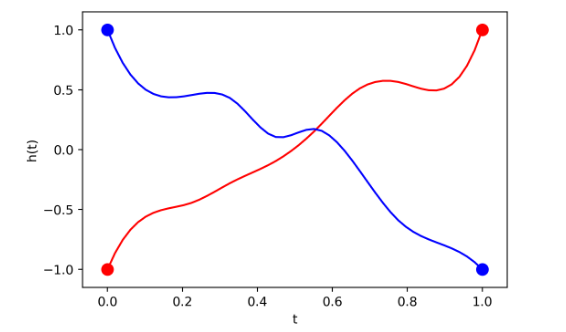
\includegraphics[width=0.4\linewidth]{left.png}
    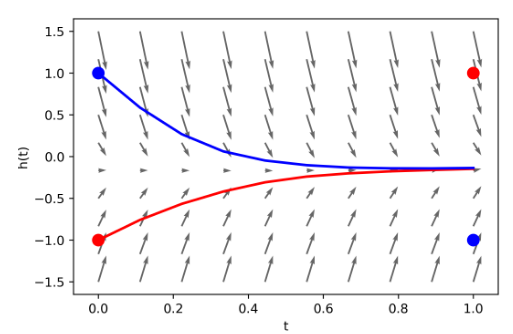
\includegraphics[width=0.4\linewidth]{right.png}
    \caption{The left graphic shows the time evolution of two example trajectories going from $1$ to $-1$(blue) and $1$ to $-1$(red). It is clear that at some point the trajectories must intersect. The right graphic shows the vector field and corresponding trajectories when one attempts to train a neural ODE on approximating the function $g$. }
    \label{fig:enter-label}
\end{figure}

Now, the argument above is just for scalar valued functions. 

\color{orange} Q1.2 (5 pts) \color{black} It is your job to extend this argument to vector valued functions. That is, find a class of functions $g: \mathbb{R}^d \to \mathbb{R}$ such that a Neural ODE (NODE) cannot represent. To do so, we define the vector valued NODE as 
\begin{align}
    \frac{d \bm{z}(t)}{dt} = \hat{\bm{f}}(\bm{z}(t), t)\,, \quad \bm{z}(0) = \bar{\bm{z}}_0    
\end{align}
where $\bar{\bm{z}}_0 \in \mathbb{R}^d$ and $\hat{\bm{f}}$ is a neural network mapping $\hat{f}: \mathbb{R}^d \times [0, T] \to \mathbb{R}^d$. Notice that $\bm{z}(T) \in \mathbb{R}^d$ and so we define the output to be $g$ to be the softmax of $\bm{z}(T)$ as if we were using a Neural ODE to preform a classification task, namely
\begin{align}
    g(\bm{x}) &= \max\{\sigma_1, \sigma_2, ..., \sigma_d\}\,, \\ 
    \sigma_i &= \frac{e^{\bm{z}_i(T)}}{\sum_{j=1}^D e^{\bm{z}_j(T)}}\,. 
\end{align}
In fact, we could choose $g(\bm{x}) = h(\bm{z}(T))$ for any continuous function $h:\mathbb{R}^d \to \mathbb{R}$ and the result would hold. 

Hint: consider functions of the form 
\begin{align}
    g(\bm{x}) = \begin{cases} 1 \text{ if }\|\bm{x}\| \text{ ...} \\ 
    -1 \text{ if }\|\bm{x}\|\text{ ...}
    \end{cases}
\end{align}
for $\bm{x} \in \mathbb{R}^d$. Explain (no need for formal proof) why such functions cannot be approximated. If you are still stuck, check out the following paper \href{https://arxiv.org/pdf/1904.01681}{Augmented Neural ODEs}.
\color{black}
\begin{tcolorbox}\centering
    Your response goes here. 
\end{tcolorbox}


\subsection{ Why? What property do neural ODEs exhibit that stops their universal approximation? (5pts)}

The key issue in the above example is that the trajectories must cross due to the fact that neural ODEs \textbf{can only perform continuous transformations} of their input data. 
To give this more formally, let us define the flow of any ODE given by  with input $\bar{\bm{z}}_0$. Recall that $\bar{\bm{z}}_0$ is the input into the neural network - ie think an image, or a list of features on an object for classification. Then, we define the flow as $\phi_t: \mathbb{R}^d \to \mathbb{R}^d$ as $\phi_t(\bm{z}_0) = \bm{z}(t)$ where $t$ is a parameter for $\phi$. 

Then, there is an important result in ODEs that says $\phi(\bar{\bm{z}}_0)$, the flow \textbf{for any ODE}, is a homeomorphism (See \href{https://en.wikipedia.org/wiki/Homeomorphism}{Wikipedia} for details on homeomorphisms if unfamiliar). In essence, homeomorphic maps are those that preserve topology, namely one can use a homeomorphic map to shape a square to a circle, but cannot shape a sphere to a torus since there is a hole in the torus and the sphere is completely connected. 

To prove this result, we will need four parts.

\begin{proposition}(Gronwall's Lemma) 
Let $U \subset \mathbb{R}^d$ be an open set. Let $f : U \times [0, T] \to \mathbb{R}^d$ be a continuous function and let $z_1, z_2: [0, T] \to U$ satisfy the initial value problems
\begin{align}
    \frac{d z_1(t)}{dt} = f(z_1(t), t), \quad z_1(0) = \bar{z}_1 \\ 
    \frac{d z_2(t)}{dt} = f(z_2(t), t), \quad z_2(0) = \bar{z}_2
\end{align}
Assume that $f$ is Lipschitz in its first argument, that is exists $C$ such that 
\begin{align}
    \|f(z_2(t), t) - f(z_1(t), t)\| \leq C \|z_2(t) - z_1(t)\|\,, \quad \forall t \in [0, T]\,.
\end{align}
Then, we have that 
\begin{align}
    \|z_2(t) - z_1(t) \| \leq e^{Ct}\|\bar{z}_2 - \bar{z}_1\|\,. 
\end{align}
\end{proposition}

% Hint: Use the property
% \begin{align}
%     \frac{d}{dt}\|z_1(t)-z_2(t)\| \leq \|z_1'(t)-z_2'(t)\|\,. 
% \end{align}
% to obtain $C$ such that 
%  \begin{align}
%         \frac{d}{dt}\|z_2(t) - z_1(t)\| - C\|z_2(t) - z_1(t)\| \leq 0 
% \end{align}. 
% Then, compute the derivative of 
% \begin{align}
%     \frac{d}{dt}(e^{-Ct}\|z_2(t)-z_1(t)\|) 
% \end{align}
% which you know must always be $\geq 0$. 
\begin{proof}
    Note that $\frac{d}{dt}\|z(t)\| \leq \|z'(t)\|$ for all functions. Thus, we have that 
    \begin{align}
        \frac{d}{dt}\|z_2(t) - z_1(t)\| &\leq \|z_2'(t) - z_1'(t)\| \nonumber  \\ 
        &= \|f(z_2(t), t) - f(z_1(t), t)\| \nonumber \\ 
        &\leq C\|z_2(t) -z_1(t)\|  
    \end{align}
    Therefore, 
    \begin{align}
        \frac{d}{dt}\|z_2(t) - z_1(t)\| - C\|z_2(t) - z_1(t)\| \leq 0 
    \end{align}
    Multiplying by $e^{-Ct}$ yields
    \begin{align}
        \frac{d}{dt}(e^{-Ct} \|z_2(t) - z_1(t)\|) \leq 0
    \end{align}
    Integrating both sides from $0$ yields
    \begin{align}
        e^{-Ct} \|z_2(t) - z_1(t)\| - \|z_2(0) - z_1(0)\| \leq 0 
    \end{align}
    Moving $\|z_2(0) - z_1(0)\|$ to the right hand side and multiply by $e^{Ct}$ yields the desired result. 
\end{proof}
\color{black}

\noindent 
Using Grownall's Lemma, prove:
\begin{proposition}
    For all $t \in [0, T]$, the flow $\phi_t:\mathbb{R}^d \to \mathbb{R}^d$ is continuous. 
\end{proposition}

\begin{proof}
    To show continuity, consider two different ODE systems with initial conditions $z_1(0) = \bm{x}$ and $z_2(0) = \bm{x}+\delta $. Then, we have via Gronwall's
    \begin{align}
        \|z_2(t) - z_1(t)\| \leq e^{Ct} \|z_2(0) - z_1(0)\| \leq e^{Ct}\|\delta\|
    \end{align}
    or in terms of $\phi_t$, we have that 
    \begin{align}
        \|\phi_t(\bm{x}+\delta) - \phi_t(\bm{x})\| \leq e^{Ct}\|\delta\| 
    \end{align}
    which as $\delta \to 0$, the right hand side moves to $0$ implying that $\phi_t$ is continuous for $\bm{x}$ for all $t \in [0, T]$. 
\end{proof}
\color{black}
\begin{proposition}
    For all $t \in [0, T]$, the flow $\phi_t:\mathbb{R}^d \to \mathbb{R}^d$ is a bijection. 
\end{proposition}

\begin{proof}
    This proof is exactly the same as Proposition 2. Assume $\phi_t(\bar{\bm{z}}_1) = \phi_t(\bar{\bm{z}}_2)$ where $\bar{\bm{z}}_1$ and $\bar{\bm{z}}_2$ are the initial conditions and $\bar{\bm{z}}_1 \neq \bar{\bm{z}}_2$. Then, consider the IVP with initial condition at $t_0$ such that $z(t_0) = \phi_t(\bar{\bm{z}}_1) = \phi_t(\bar{\bm{z}}_2)$. By Proposition 1, if we solve this ODE backward in time, the solution is unique and therefore it is not possible to map to two different $\bar{\bm{z}}_1$ and $\bar{\bm{z}}_2$. Therefore, we must have that if $\bar{\bm{z}}_1 \neq \bar{\bm{z}}_2$, then $\phi_t(\bar{\bm{z}}_1) \neq \phi_t(\bar{\bm{z}}_2)$ and so the $\phi_t(\bm{z})$ is one-to-one.  
\end{proof}
\color{black}

\begin{proposition}
     For all $t \in [0, T]$, the inverse flow $\phi_t^{-1}:\mathbb{R}^d \to \mathbb{R}^d$ is also continuous. 
\end{proposition}

\begin{proof}
    $\phi_t^{-1}$ is continuous since we can set the initial condition of the ODE to be $\phi_t(\bar{\bm{z}})$ and then solve backward in time applying the same technique as Proposition 4. 
\end{proof}
\color{black}
\begin{corollary}
    Then, by Proposition 4, 5, and 6, for all $t \in [0, T]$, the flow $\phi_t: \mathbb{R}^d \to \mathbb{R}^d$ is a homeomorphism. That is, it preserves the topology of the underlying space!
\end{corollary}

Since all ODE feature maps $\phi(\bar{\bm{z}}_0)$ are homeomorphism, that includes those of Neural ODEs and therefore, they are unable to approximate functions that change the underlying topology of the input feature vector. However, we can alleviate this. Instead of defining the input vector as just the $d$ dimensional feature vector, we introduce the $\textbf{augmented}$ neural ODE framework, namely
\begin{align}
    \frac{d}{dt}\begin{bmatrix}
        \bm{z}(t) \\ \bm{a}(t) 
    \end{bmatrix} = \hat{\bm{f}}(\begin{bmatrix} \bm{z}(t) \\ \bm{a}(t) \end{bmatrix}, t ), \quad \begin{bmatrix} \bm{z}(0) \\ \bm{a}(0) \end{bmatrix} = \begin{bmatrix} \bar{\bm{z}}_0 \\ \bm{0} \end{bmatrix}
\end{align}
where $\bm{a}(t) \in \mathbb{R}^d$ for all $t \in [0, T]$. That, is we extend the neural ODE with a zero input length of size $d$ and learn the mapping above with $\bm{a}(T) = 0$. 

By introducing the extra dimension, this allows the flows to never ``cross" as they use the extra topology to differentiate themselves. For example, as above, lets assume that $z_1(\bar{t}) = z_2(\bar{t})$, that is $\bar{t}$ is the point in the left of Figure \ref{fig:enter-label} where the trajectories cross. Now, using the augmented neural ode, we choose the augmented states to differ between $\bm{z}_1$ and $\bm{z}_2$ such that the function can now be approximated by $\hat{f}$! The question is, is this trick enough? That is, does it enable neural ODEs to be universal approximators. The answer is of course yes! For those who are interested, the proof is given in \href{https://arxiv.org/pdf/2202.02435}{this paper}  - See Section 3.2. 

Lastly, we finish with an empirical question. That is, what does this mean for the practitioner? In essence, we have learned that neural ODEs can struggle, but augmented neural ODEs can alleviate this issue. 

\color{orange} Q1.3 (5 pts) \color{black} Give an example of a real-world classification task where augmented Neural ODEs outperform traditional Neural ODEs. Explain the task (5pts) as well as why the performance would be better from a function approximation perspective (Bonus 5pts) (Hint: Consider any \emph{non-linear} classification tasks where the regular Neural ODE has the same dimension as the number of categories as the classifier. Can you make any connection to kernels in support vector machines?) 

\begin{tcolorbox}\centering
    Your response goes here. 
\end{tcolorbox}

 
 Now, go experiment with augmented neural ODEs in the coding portion of the homework! You may find \href{https://arxiv.org/abs/1904.01681}{this paper} useful in your implementation. 

\section{Neural ODEs: Coding Section (30pts)}
For the entire coding section, you can use PyTorch as well as other standard packages (NumPy, Scikit-learn, ect.)

\color{orange} Q2.1 Implement a Multi-Layer Perceptron (5pts) \color{black} Implement a classic MLP. The inputs to your network will be both $x$, your set of data, as well as $t$ to make a time dependent MLP. In order to make the dimension fit, you will repeat $t$ the dimension of $x$ times and concatenate them so your input into your MLP is $(x, t)$. We leave the choice of number of layers, hidden dimension and activation function up to you. 

To test your approach, we give a simple dataset that learns the function $f(x, t) = ax^2 + bx+ct$ with parameters $a, b$ and $c$ unknown. The goal of your neural network is to take a random input $x, t \in [-10, 10] \times \{10\}$ and output $f(x, t)$. One must achieve a test loss of $2 \times 10^{-3}$ as given in the test to receive full credit.  

\color{orange} Q2.2 Implement a Neural ODE (5pts) \color{black} To implement a Neural ODE, we have broken up the problem into two parts. The first part, denoted by the class NeuralODEBlock will control a single neural ODE layer where as the second block NeuralODE will combine the neural ODE layers with your MLP class.  

For the NeuralODEBlock, we ask you to implement two methods in the class. The first method computes the forward path of which you can use `odeint` from torchdiffeq. This is a differentiable ODE solver and is the \emph{only method} you are allowed to use from torchdiffeq. For the method in the odeint solver, please choose `dopri5` which is a classic ODE solver method. Use the tolerance given for both tolerances and set the max steps parameter as well. 

You should be able to obtain an extremely accurate loss $10^{-7}$ with very few epochs on the simple dataset, but fail to obtain anything useful on the non-simple dataset. Ensure that your plots are visible as these should show correct and incorrect trajectories and count for a 2pts each. 

\color{orange} Q2.3 Implement an Augmented Neural ODE (5pts) \color{black}
In this section you will create an augmented neural ODE where you increase the dimension of $x$ by one and then learn the ODE as discussed above where the augmented state is $0$ at the initial and final times of the ODE. You again can use `odeint` for this class. 

This time, when training on the hard dataset, you should find the augmented Neural ODE can do extremely well - achieving errors on the magnitude of $10^{-5}$. 

\color{orange} Q2.4 Discussion (15pts). \color{black} Please provide your answers below. Each question is worth 5pts.
\begin{enumerate}
    \item Give an interpretation of this vector field and what you make of it. What would be a better way to plot it? Respond \underline{in the Jupyter notebook}.

     \item Why does the augmented Neural ODE work? Discuss the pros and cons of this approach. Respond \underline{in the Jupyter notebook}.

     \item You made a series of design decisions at each step from the MLP to Neural ODE.  Discuss these decisions including your choice of parameters and what fundamental ideas in ML influenced your choices (bias/variance tradeoff, regularization, etc.) Respond \underline{in the Jupyter notebook}.

\end{enumerate}

\section{Neural Operators: How do we build datasets for PDEs (30pts)}
Before discussing neural operators and learning the solution mappings to PDEs, we should understand \emph{why do we even need a deep learning framework to solve these equations}? In this section, we will discuss the common methods for simulating PDEs and you will derive a finite difference scheme for the 1D Burger's equation. 

\subsection{Burger's Equation}
The Burger's equation is a fundamental equation in PDEs that describes phenomena ranging from fluid mechanics to shock waves to traffic flow. It is perhaps the simplest nonlinear-PDE and will be the PDE we explore throughout the rest of this homework. We will consider the Burger's equation of the form
\begin{subequations}\label{eq:burgers}
    \begin{align}
    u_t(x, t) + u u_x(x, t) - \nu u_{xx} &= 0\,, \quad x \in [-1, 1]
, \quad t \in [0, 1 ] 
\\  
u(0, x) &= \phi(x, k_1, k_2)\,, \\
u(t, -1) = u(t, 1) &= 0\,. \label{eq:burgers_bc} 
\end{align}
\end{subequations}
where $\phi(x, k_1, k_2)$ is given below in the coding section and is not needed for this portion. This PDE represents the diffusion of a shock wave and is good for modeling an earthquake like the one we had a few weeks ago. That is, starting from some large initial shock, how will the wave propagate to its neighbors? 

\color{black}

In this section, we will answer the question:
\begin{tcolorbox} \centering
\textbf{How to simulate this PDE in practice on a computer?}
\end{tcolorbox}

\subsection{Approximating derivatives in practice: Finite Difference Method (30pts)}
First, note that the PDE \eqref{eq:burgers} is represented in a continuous form of which a computer cannot handle. Thus, to simulate this type of PDE on a computer, we need to use an approximation of the continuous components, or the derivatives. As discussed in the PDE review, we can use the approach of finite differencing. Thus, we derive two finite differencing schemes. 

\color{orange} Q3.1 (5 pts) \color{black} Derive finite difference schemes for approximating the derivatives $u_t$, $u_x$ using the function values $u(x, t), u(x, t+\delta t), u(x+\delta x, t)$, where $\delta x, \delta t$ are the spatial and temporal discretizations sizes.

Hint: First-order Taylor expansion for function value at $u(x, t+\delta t)$ is given by: $u(x, t+\delta t) = u(x, t) + \delta t \cdot u_t(x, t) + O((\delta t)^2)$ and first-order Taylor expansion for function value at $u(x+\delta x, t)$ is given by: $u(x+\delta x, t) = u(x, t) + \delta x \cdot u_x(x, t) + O((\delta x)^2)$. 

\begin{tcolorbox}\centering
    Your response goes here. 
\end{tcolorbox}

\color{black}
\color{orange} Q3.2 (5pts) \color{black} Using the previous results, derive a finite difference approximation for the second-order spatial derivative $u_{xx}$ using a Taylor expansion of $u_x(x+\delta x, t)$. 
\begin{tcolorbox}\centering
    Your response goes here. 
\end{tcolorbox}
\color{black}

\color{orange} Q3.3 (5pts) \color{black} Using your finite difference approximations for the partial derivatives $u_t, u_x, u_{xx}$ derived above, derive a finite difference solution scheme for the Burger's equation. Start with initial condition $u(0, x) = \phi(x, k_1, k_2)$ and enforce the boundary conditions given in \eqref{eq:burgers_bc}.
\begin{tcolorbox}\centering
    Your response goes here. 
\end{tcolorbox}
\color{black}

\subsection{Under what conditions, does a finite difference scheme become numerically stable? (5pts)}

\color{orange} Q3.4 (5pts) \color{black} The finite difference schemes only accurately approximate the derivatives when $\delta t$ and $\delta x$ are small. Why?
\begin{tcolorbox}\centering
    Your response goes here. 
\end{tcolorbox}
\color{black} 

The condition that $\delta x$ and $\delta t$ typically need to satisfy is called the \href{https://en.wikipedia.org/wiki/Courant%E2%80%93Friedrichs%E2%80%93Lewy_condition}{Courant-Freidrichs-Lewy}
(CFL) condition, and it varies for each type of PDE. Unfortunately, for the Burger's equation in this example, due to the nonlinearity, it is not possible to derive the condition. Therefore, it is up to the \emph{user} to identify good choices for $\delta t$ and $\delta x$. Typically, it is expected that $\delta t \ll \delta x$ and one tries to choose $\delta x$ small enough that there are enough spatial steps to capture the rich behavior. Reasonable choices are $\delta x = 0.05$ and $\delta t=0.001$ which would result in $T / \delta t * (2/\delta x)$ or for $T = 5$, $200k$ different points in the discretization grid. Clearly, this will become numerically expensive extremely quickly. Hence, it is reasonable to look for \emph{discretization invariant} approaches using the tool of machine learning! This is why the neural operator approach is so powerful. 

\subsection{Finite Differencing: Coding Section (10pts)}
In this section, we will implement your finite difference scheme and later use it to build a neural operator approximation. In particular, we will consider two different datasets of the Burger's condition with the following initial $(x \in [-2\pi, 2\pi])$ and boundary conditions:
\begin{align}
    u(-2\pi,  t) &= u(2\pi, t) = 0\,, \quad t \in (0, 5)\,, \label{eq:bc-1}   \\
    u(x, 0) & = \phi(x, k_1, k_2)\,, \quad x\in (-2\pi, 2\pi)\,, \label{eq:ic-1}  \\
    \phi(x, k_1, k_2) &= e^{-(x-k_1)^2 / 4 \nu} - e^{-(x+k_2)^2 / 4 \nu}\,, \quad k_1, k_2 \in [0, \pi/2]\,, \label{eq:ic-2}
\end{align}
with the viscosity large as $\nu=0.1$. 
Notice, the variables $k_1, k_2$ modify our initial condition and we will use this single parameter to build a dataset. Further, notice the initial condition is the sum of two Gaussians - can you guess what it may look like (answer below)? 

\color{orange} Q3.5 (5pts)\color{black} Generate a plot of the initial condition for a couple $k_1, k_2$ \underline{in the Jupyter notebook}. Comment on what happens when $k_1 = k_2$ (e.g. $k_1 = k_2 = \pi/2 $) and when $k_1 \gg k_2$ (e.g. $k_1 = \pi/2, k_2 =  1 \times 10^{-2}$)? 


\color{orange} Q3.6 (5pts) \color{black} Plot the value of the PDE system at $t=5$ for both initial conditions in Q4.1 \underline{in the Jupyter notebook}. Use one plot with a legend as in the initial condition. You must also past the test\_pde function to receive full points in the notebook section. 
\color{black}


\section{Neural Operators: Coding Section (25 points)}
In this section, we will explore the super-resolution property of neural operators. 
We have created two different datasets for you corresponding to the Burger's equation \eqref{eq:burgers}, \eqref{eq:burgers_bc} with the initial and boundary conditions given as in \eqref{eq:bc-1}, \eqref{eq:ic-1}, \eqref{eq:ic-2}. The inputs in the dataset are parameterizations of $\phi$ with values of $k_1, k_2$ uniformly distributed between $[0, \pi]$ and the outputs are the corresponding value of the PDE at time $t=5$. The difference between the datasets are the chosen discretization sizes. In particular, for the first dataset, we consider $dt=0.05$ and $dx=0.1$ -  a very coarse resolution while in the second dataset, we consider $dx=0.05$ and $dt=0.01$ - a much more refined grid.

\color{orange} Q4.1 (5pts) \color{black} How many points are required to simulate each grid to $T = 5$ seconds including the endpoints at $t=0$ as well as $x=-2\pi, 2\pi$ (round to nearest whole number)? 
 \begin{tcolorbox}\centering
    Your response goes here. 
\end{tcolorbox}

\color{orange} Q4.2 (10pts) \color{black} Implement a FNO as discussed in class. To do this, we ask you to implement two parts. The SpectralConv class which performs an FFT, multiplies by a weight matrix and then performs and IFFT. You can use torch.rfft and torch.irfft for the Fast Fourier Transform. 

Then, we ask you to combine this SpectralConv class with a series of MLP layers as discuss to make a Fourier Neural Operator. You may find Figure 2 of \url{https://arxiv.org/pdf/2010.08895} helpful.  

Your resulting FNO should recieve test errors of $3 \times 10^{-4}$ on both datasets to receive all points. 

\color{orange} Q4.3 (5pts) \color{black} Qualitatively and quantitatively compare the super-resolution property of your FNO. Briefly comment \underline{in the Jupyter notebook} on your performance both qualitatively and quantitatively. Is it as expected? 

\color{orange} Q4.4 (5pts) \color{black} Add a physics informed loss to your FNO. Since we have a time-derivative based PDE and we only want to consider the output at a single point, we cannot encode the PDE solution completely. However, we can ensure soft-regularization of the boundary conditions. Thus, modify the training loss to 
\begin{align*}
    \text{Loss}(y, \hat{y}) = \|y - \hat{y}\|_{L^2} + \lambda_1 |\hat{y}(-2\pi)-0|  + \lambda_2 |\hat{y} (2\pi) -0|\,. 
\end{align*}
where you choose the parameter values of $\lambda_1$, $\lambda_2$. Again explore the behavior of the FNO and it super-resolution capability. 

Briefly comment \underline{in the Jupyter notebook} on the results. Are your models more accurate? Less? Why do you think? How does the super-resolution result change? Any qualitative notes? How did you choose $\lambda_1, \lambda_2$? Do they matter a lot?
\end{document}

